\documentclass[12pt]{ruthesis}
\usepackage{amsmath}
\usepackage{amssymb}
\usepackage{array}
\usepackage{longtable}
\usepackage{tabularx}
\usepackage{multirow}
\usepackage{rotating}
\usepackage{booktabs}
\usepackage{tablefootnote}
\usepackage{mathtools}
\usepackage{physics}
\usepackage{adjustbox}
\usepackage{float}
\usepackage{graphicx}
\usepackage[inkscapelatex=false]{svg}
\usepackage[hyperfootnotes=true]{hyperref}
\usepackage{color}
\usepackage{bm}
\usepackage[]{siunitx}
\usepackage[]{cleveref}
\usepackage[style=phys,
			articletitle=true,
			hyperref=true,
			biblabel=brackets,
			chaptertitle=false,
			pageranges=false,
			backend=biber]{biblatex}

%%%%%%%%%%%%%%%%%%%%%%%%%%%%%%%%%%%%%%%%%%%%%%%%%%%%%%%%%%%%%%%%%%%
%%%%	Various options
%%%%%%%%%%%%%%%%%%%%%%%%%%%%%%%%%%%%%%%%%%%%%%%%%%%%%%%%%%%%%%%%%%%
\addbibresource{bibliography.bib}

\graphicspath{{chapters/},
			  {appendices/}}

\svgpath{{chapters/},
		 {appendices/}}

% Footnotes are continuously labeled (e.g. without regard for sections, chapters, etc.). 
\usepackage{chngcntr}
\counterwithout{footnote}{chapter}
\interfootnotelinepenalty=10000 %Supposed to keep footnotes from being split

% Additional options
\DeclareSIUnit\atoms{atoms}

% cleveref options (\Cref{} for start of sentence, \cref{} for abbreviation).
\Crefname{equation}{Equation}{Equations}
\crefname{equation}{Eq.}{Eqs.}
\Crefname{figure}{Figure}{Figures}
\crefname{figure}{Fig.}{Figs.}
\Crefname{table}{Table}{Tables}
\crefname{table}{Tab.}{Tab.}

% Allows setting l, c, r column widths (needs tabularx)
\newcolumntype{L}[1]{>{\raggedright\arraybackslash}p{#1}}
\newcolumntype{C}[1]{>{\centering\arraybackslash}p{#1}}
\newcolumntype{R}[1]{>{\raggedleft\arraybackslash}p{#1}}


%%%%%%%%%%%%%%%%%%%%%%%%%%%%%%%%%%%%%%%%%%%%%%%%%%%%%%%%%%%%%%%%%%%
%%%%	Macros
%%%%%%%%%%%%%%%%%%%%%%%%%%%%%%%%%%%%%%%%%%%%%%%%%%%%%%%%%%%%%%%%%%%
% Making a command equivalent to \adjustimage but for svg
\newcommand{\adjustsvg}[2]{\adjustbox{#1}{\includesvg{#2}}}

\newcommand{\RomanNumeralCaps}[1]{\MakeUppercase{\romannumeral #1}}

\newcommand{\Sri}{Sr \RomanNumeralCaps{1}}
\newcommand{\Srii}{Sr \RomanNumeralCaps{2}}

\newcommand{\tsup}{\textsuperscript}								% superscript outside math mode.
\newcommand{\tsub}{\textsubscript}									% subscript outside math mode.
\newcommand{\Sr}[1]{\tsup{#1}\text{Sr}}								% ^{8x}Sr outside math mode.
\newcommand{\Srion}[2]{\Sr{#1}\tsup{#2}}							% ^{8x}Sr^{x+} outside math mode.
\newcommand{\Li}[1]{\tsup{#1}{Li}}									% ^{xx}Li outside math mode.

\newcommand{\SLJ}[3]{\tsup{#1}{#2}\tsub{#3}}
\newcommand{\SLJm}[4]{\SLJ{#1}{#2}{#3}{,\,}{m_J = {#4}}}
\newcommand{\SLJF}[4]{\SLJ{#1}{#2}{#3}{,\,}{F = {#4}}}
\newcommand{\nSLJ}[4]{({#1}){\,}\SLJ{#2}{#3}{#4}}
\newcommand{\nSLJm}[5]{\nSLJ{#1}{#2}{#3}{#4}{,\,}{m_J = {#5}}}
\newcommand{\nSLJF}[5]{\nSLJ{#1}{#2}{#3}{#4}{,\,}{F = {#5}}}
\newcommand{\nSLJFm}[6]{\nSLJ{#1}{#2}{#3}{#4}{,\,}{F = {#5}}{,\,}{m_F = {#6}}}

\newcommand{\iu}{{i\mkern1mu}}	% i for imaginary unit

% 3j, 6j symbols
\newcommand{\threej}[6]{
	\begin{pmatrix}
		#1 & #2 & #3 \\
		#4 & #5 & #6 
	\end{pmatrix}}

\newcommand{\sixj}[6]{
	\begin{Bmatrix}
		#1 & #2 & #3 \\
		#4 & #5 & #6 
	\end{Bmatrix}}

%%%%%%%%%%%%%%%%%%%%%%%%%%%%%%%%%%%%%%%%%%%%%%%%%%%%%%%%%%%%%%%%%%%
%%%%	Front-matter details
%%%%%%%%%%%%%%%%%%%%%%%%%%%%%%%%%%%%%%%%%%%%%%%%%%%%%%%%%%%%%%%%%%%

\title{PhD Thesis Title Here}
\author{Roger Ding}
\department{Applied Physics}
\school{William Marsh Rice University}
\degree{Doctor of Philosophy}

\committee{
	F. Barry Dunning, Advisor \\
	Sam and Helen Worden Professor of Physics
	\and
	Thomas C. Killian, Co-advisor \\
	Professor of Physics and Astronomy
	\and
	Junichiro Kono \\
	Professor of Electrical and Computer Engineering \\
	Professor of Physics and Astronomy
	\and
	Han Pu \\
	Professor of Physics and Astronomy
}

\address{Houston, Texas}
\donemonth{April}
\doneyear{2019}
\makeindex

\begin{document}

%%%%%%%%%%%%%%%%%%%%%%%%%%%%%%%%%%%%%%%%%%%%%%%%%%%%%%%%%%%%%%%%%%%
%%%%	Front-matter
%%%%%%%%%%%%%%%%%%%%%%%%%%%%%%%%%%%%%%%%%%%%%%%%%%%%%%%%%%%%%%%%%%%

\begin{frontmatter}
	\pagenumbering{roman}
	%\makecover
	\maketitle
	This dissertation describes the development of an apparatus to undertake spectroscopic studies of \Sr{87} Rydberg states and their application in the production of ultra-long-range Rydberg molecules (ULRRMs). 
Most previous spectroscopic studies of strontium have been performed with the bosonic isotope \Sr{88} which has no nuclear spin ($I = 0$), resulting in a relatively simple and well-understood Rydberg excitation spectrum. 
In contrast, fermionic \Sr{87} has a large nuclear spin ($I = {9}/{2}$) that leads to strong hyperfine interactions which greatly complicate the Rydberg excitation spectrum.
In order to understand the Rydberg states in \Sr{87}, two-photon spectroscopy was performed to measure and identify the $\nSLJ{5sns}{3}{S}{}$ and $\nSLJ{5snd}{3}{D}{}$ hyperfine Rydberg states for $30 \lesssim n \lesssim 99$.
Working with theory collaborators, a detailed understanding of how the hyperfine interaction affects the Rydberg levels is developed and used to extract revised quantum defects.

The detailed understanding of the \Sr{87} hyperfine Rydberg structure was then utilized to produce the first ULRRMs in a fermionic gas.
Unlike traditional molecular binding mechanisms, ULRRMs comprise of one or more ground-state atoms embedded in the electron cloud of a Rydberg atom with the entire system bound together through the weak Rydberg electron-neutral atom scattering. 
Therefore, production of ULRRMs is dependent on both the principal quantum number ($n$) of the parent Rydberg atom and the initial spatial distribution of atoms. 
At low temperatures, the effects of quantum statistics becomes important and result in bunching (bosons) and antibunching (fermions).
These differences in spatial distributions can influence the excitation rates of ULRRMs. 
Current progress in exploring the role of quantum statistics in the excitation of ULRRMs using cold, dense strontium gases is described, with an emphasis on \Sr{87}, and how such measurements can be used to extract the pair correlation function $g^{\pqty*{2}}\pqty*{R}$.
	\begin{acknowledge}

Acknowledgments go here. 

\end{acknowledge}
	\tableofcontents
	\listoffigures
	\listoftables
\end{frontmatter}

\pagenumbering{arabic}

\linespacing{1.7}

%%%%%%%%%%%%%%%%%%%%%%%%%%%%%%%%%%%%%%%%%%%%%%%%%%%%%%%%%%%%%%%%%%%
%%%%	Chapters
%%%%%%%%%%%%%%%%%%%%%%%%%%%%%%%%%%%%%%%%%%%%%%%%%%%%%%%%%%%%%%%%%%%

\chapter{Introduction}

***************************************************

*********** NOTES TO SELF, REMOVE LATER ***********

(0) Long-range and anisotropic interactions

(0a) Few-/Many-body physics

(0b) Ultra-long-range Rydberg molecules

(1) Spectroscopy

(2) Effects of quantum statistics -- use Joe's figure?

Add in repumper spectrum.

***************************************************

***************************************************



The ability to produce ultracold samples paved the way towards achievement of quantum degenerate gases of atoms which are ideal systems for studying quantum interactions. 
From the observation of BEC-BCS crossover \cite{Chen2005.PR.412.1, Gurarie2007.JAOP.322.2, Bourdel2004.PRL.93.050401}, superfluid to Mott insulator transition in an optical lattice \cite{Greiner2002.Nature.415.39}, and the formation of matter-wave solitons \cite{Strecker2002.Nature.417.150, Khaykovich2002.Science.296.1290}, most of the work in these systems have been based on a short-range, isotropic contact interactions described by the pseudopotential \cite{Pethick.BEC}
\begin{equation}
	U\pqty{\va{r}}	=	\frac{4 \pi \hbar^2}{m} a_{s} \delta\pqty{\va{r}}
\end{equation}
where $a_{s}$ is the $s$-wave scattering length.
This effective interaction requires the atomic wave functions to overlap. 

An important recent trend in the field of ultracold atomic gases is the study of systems with long-range interactions which can typically be expanded as \cite{Pethick.BEC}
\begin{equation}
	U\pqty{\va{r}}	=	\sum^{\infty}_{k=1} \frac{C_{k} \pqty{\va{r}}}{r^{k}}
\end{equation}
with the ``long-range'' coming from the $U \sim {1}/{r^{k}}$ dependence. 
Depending on the type of interaction (e.g., Coulomb $k = 1$, dipole-dipole $k = 3$, van der Waals $k = 6$), the potentials can be isotropic or anisotropic, providing additional richness to quantum systems and the opportunity to study a wide variety of phenomena including applications towards quantum computing \cite{Jaksch2000.PRL.85.2208, DeMille2002.88.067901}, quantum simulation \cite{deLeseleuc2018.PRL.120.113602, Schauss2018.QST.3.023001}, and tests of theories **** SOURCES? ****
There are several methods for incorporating long-range interactions in to ultracold systems with some of the most prominent being \cite{Lahaye2009.RPP.72.126401}: 
\begin{description}
	\item[Polar molecules]
		These molecules can have large (permanent) electric dipole moments \cite{Aymar2005.JCP.122.204302} and can, ignoring chemical reactions, have extremely long lifetimes. 
		The drawback is that the additional complexity typically makes it very difficult to produce ultracold and quantum degenerate samples. 
		In spite of these challenges, a degenerate Fermi gas of {{\tsup{40}\text{K}}{\tsup{87}\text{Rb}}} was recently achieved by associating atoms from a BEC of {\tsup{87}\text{Rb}} and a degenerate Fermi gas of {\tsup{40}\text{K}} \cite{DeMarco2019.Science.363.853}. 
		Steady progress continues to be made in the direct laser cooling of molecules as well \cite{Anderegg2018.NatPhys.14.890}.
	\item[Magnetic atoms]
		Atoms themselves can have permanent dipole moments which can be exploited to study long-range interactions. 
		Quantum degeneracy has been reached with chromium \cite{Griesmaier2005.PRL.94.160401, Naylor2015.PRA.91.011603}, erbium \cite{Aikawa2012.PRL.108.210401, Aikawa2014.PRL.112.010404}, and dysprosium \cite{Lu2011.PRL.107.190401, Lu2012.PRL.108.215301}.
		Although simpler than molecules, their dipolar interactions are limited by the magnetic moment of atoms and typically requires tuning the short-range interaction strength to be weaker than the dipole-dipole interaction to observe their effects.
		There's also been a recent proposal for creating ultracold dysprosium atoms which exhibit an electric dipole moment in addition to the magnetic dipole moment \cite{Lepers2018.PRL.121.063201}.
	\item[Coupling atoms to a high-finesse cavity]
		An ingenious way of inducing long-range interactions in atomic systems is by placing the atoms in a high-finesse optical cavity such that they couple to the cavity mode which in turn causes the atoms to experience position-based forces \cite{Baumann2010.Nature.464.1301, Mottl2012.Science.336.1570}.
		Although the interactions are (essentially) infinite-range, they are likely to be restricted to only that case. 
		They are also constrained by the geometry of the experiment which could make it difficult to tune between isotropic and anisotropic interactions.
	\item[Rydberg states]
		Highly excited Rydberg states of atoms (and molecules) with principal quantum number $n \gg 1$ can also exhibit strong dipole interactions \cite{Gallagher1994.RydbergAtoms} and have even been observed in solid state systems \cite{Kazimierczuk2014.Nature.514.343}. 
		Since many of the properties of Rydberg atoms scale with $n$, the Rydberg-Rydberg interactions can be tuned in strength and anisotropy by simply exciting different Rydberg states. 
		Rydberg atoms can also leverage well-established techniques for producing quantum degenerate gases of atoms so that their interactions can be readily incorporated to existing setups. 
		The major disadvantage of Rydberg systems are their sensitivities to stray electric fields and the limited Rydberg lifetimes due to both blackbody and Rydberg-Rydberg interactions. 
\end{description}
This thesis will be focused on the latter by studying Rydberg systems in ultracold strontium gases. 
Most ultracold Rydberg experiments have predominantly focused on exciting alkali metal atoms (primarily rubidium and cesium with a growing interest in potassium).
With their hydrogen-like electronic structure, there are well-established methods for both calculating their properties (e.g., see \cite{Sibalic2017.CPC.220.319}) and techniques for producing ultracold and quantum degenerate gases.
But since the interactions are long-ranged, generally comparable to the inter-particle separation in the gas, the particular atomic species used should only affect the details of the interactions but not the overall form. 
As will be discussed below, strontium has some properties which make it a very advantageous system for studying Rydberg physics. 

\section{Rydberg Atoms}

A Rydberg atom can be loosely defined as an atom in an excited state with very large principal quantum number ($n$), i.e., $n \gg 1$. 
Starting in the late {1800's}, it was observed that the wavenumbers of atomic spectra could be described by the formula
\begin{equation}
	\label{eq:Rydberg_formula}
	\nu_{l} = \nu_{\infty,l} - \frac{R}{\pqty{n-\delta_{n,l}}^2}
\end{equation}
where $\nu_{\infty,l}$ is the series limit, $\delta_{n,l}$ is a ``quantum defect'', and $R$ is the Rydberg constant \cite{Rydberg1890.Recherches, Rydberg1890.PM.29.331, Gallagher1994.RydbergAtoms}. 
This is the Rydberg formula.
Conceptually, a Rydberg atom can be thought of as being comprised of a core ion and a highly-excited valence electron which spends the majority of its time far away from the core.
As a result, the Rydberg electron rarely interacts with the core which allows its effects to be characterized by (nearly) constant parameter $\delta_{n,l}$.
While the details of the core ion and electrons are important, which causes $\delta_{n,l}$ to vary from atom-to-atom and from orbital-to-orbital, it generally does not have a large effect on the overall properties of the Rydberg atom.

Although the details of the core are usually small, the principal quantum number does greatly affects the atomic wave function. 
As a result, it sets the energy scale for many interactions which leads to the properties of Rydberg atoms become exaggerated when $n$ becomes large.
\Cref{tab:Rydberg_n-scaling} gives the $n$ dependence for a few Rydberg atoms properties. 
\begin{table}[h]
	\centering
	\caption[]{
		\label{tab:Rydberg_n-scaling}
		Some properties of Rydberg atoms \cite{Gallagher1988.RPP.51.143, Gallagher1994.RydbergAtoms, Camargo2016.PRA.93.022702, Ding2018.PRA.98.042505}.
		*** Double check values!! ***}
	\begin{tabular}{@{}cccc@{}}
		\toprule
		Property					& $n$ scaling	& {Na} : {$\nSLJ{10d}{2}{D}{}$}					& {Sr} : {$\nSLJ{5s38s}{3}{S}{1}$}	\\
		\midrule
		Binding energy				& $n^{-2}$		& $\SI{0.14}{\eV}$								& $\SI{0.01134}{\eV}$				\\
		Coulomb splitting			& $n^{-3}$		& $\SI{0.023}{\eV}$								& $\SI{0.00058}{\eV}$				\\
		Fine structure splitting	& $n^{-3}$		& $\SI{-92}{\MHz}$								& $\SI{2.56659}{\GHz}$				\\
		Orbital radius				& $n^{2}$		& $\SI{147}{\bohr}$								& $\SI{1799}{\bohr}$				\\
		Radiative lifetime			& $n^{3}$		& $\SI{1}{\us}$									& $\SI{21}{\us}$					\\
		Polarizability				& $n^{7}$		& $\SI{0.21}{\MHz\per(\volt\per\cm)\squared}$	& 									\\
		Ionization field			& $n^{??}$		&												& 									\\
		\bottomrule
	\end{tabular}
\end{table}

\subsection{Ultralong-Range Rydberg Molecules (ULRRMs)}

One key aspect to focus on from \cref{tab:Rydberg_n-scaling} is that size of a Rydberg atom increases very quickly with $n$. 
In a dense enough gas, $\ev*{r} \sim n^{2}$ can quickly become comparable to (or larger than) the interparticle separations.
It was in this context, when an atom (or multiple atoms) could be located inside the Rydberg electron's orbit, that a density-dependent shift was first observed in the spectral lines of alkali atoms with the direction of the shift, relative to the unperturbed atomic line, also depended on the buffer gas used \cite{Amaldi1934.NC.11.145, Amaldi1934.Nature.133.141, Liebisch2016.JPB.49.182001, Shaffer2018.NatComm.9.1965}.
\begin{figure}[htbp]
	\centering
	\includegraphics[keepaspectratio, width=\textwidth, height=\textheight]{introduction/rydberg_molecules/orbital_radius-density_n-scaling.pdf}
	\caption[]{
		\label{fig:orbital_radius-density_n-scaling}
		Orbital radius $\ev{r}$ and the corresponding density ${1}/{\ev{r}^3}$ for a strontium Rydberg atom in the $\nSLJ{5sns}{3}{S}{1}$ state.
		The shaded region represents the range of densities typically achievable in ultracold strontium experiments with a maximum of about $\SI{1E15}{\per\cm\cubed}$ occurring in a \Sr{88} BEC \cite{Yan2013.PRL.110.123201, Stellmer2014.arXiv.1307.0601}.}
\end{figure}
\Cref{fig:orbital_radius-density_n-scaling} shows $\ev{r}$ and ${1}/{\ev{r}^3}$ for a strontium atom in the $\nSLJ{5sns}{3}{S}{1}$ state and the typical densities achievable in ultracold gas experiments.
Notice that, even for modest principal quantum numbers and densities, it's easily possible to excite Rydberg atoms much larger than the interparticle separations.

This shift was first explained by Fermi \cite{Fermi1934.NC.11.157}, and later generalized by Omont \cite{Omont1977.JPF.38.1343}, to be the result of low-energy scattering of the Rydberg electron off nearby neutral atoms, formulating the electron-atom interaction with the pseudopotential \cite{DeSalvo2015.PRA.92.031403, Liebisch2016.JPB.49.182001, Shaffer2018.NatComm.9.1965}
\begin{equation}
	V\pqty*{\va{R}}
		=	\sum_{i} \frac{2 \pi \hbar^{2} A_{s}\bqty*{k\pqty*{\va{R}}}}{m_{e}} \delta\pqty*{\va{r}_i - \va{R}}
			+ \frac{6 \pi \hbar^{2} A_{p}^{3}\bqty*{k\pqty*{\va{R}}}}{m_{e}} \overleftarrow{\grad}{\delta\pqty*{\va{r}_i - \va{R}}}\overrightarrow{\grad}
\end{equation}
where $\va{r}_{i}$ is the position of the Rydberg valence electron(s) and $\va{R}$ is the position of the ground-state atom from the Rydberg core. 
On the right hand side, the first term is the $s$-wave contribution and the second term is the $p$-wave contribution with momentum-dependent scattering lengths $A_{s}\pqty{k}$ and $A_{p}\pqty{k}$, respectively, and the semiclassical Rydberg electron momentum given by $\hbar {k \pqty{\va{r}}} = \sqrt{2 m_{e} \bqty{{e^2}/{\pqty{4 \pi \epsilon_0 \va{r}}} - E_{b}}}$ for the unperturbed Rydberg electron binding energy $E_{b}$ \cite{DeSalvo2015.PRA.92.031403}.
Evaluating the interaction with the Rydberg electron wave function $\Psi_{ns}$ leads to \cite{DeSalvo2015.PRA.92.031403}
\begin{equation}
	V\pqty*{\va{R}}
		\simeq	\sum_{i} \frac{2 \pi \hbar^{2} A_{s}\pqty*{k}}{m_{e}} {\abs*{\Psi_{ns}\pqty*{\va{r}_{i} = \va{R}}}^2}
				+ \frac{6 \pi \hbar^{2} A_{p}^{2}\pqty*{k}}{m_{e}} {\abs*{\grad \Psi_{ns}\pqty*{\va{r}_{i} = \va{R}}}^2}
\end{equation}
**** NEED TO DOUBLE CHECK THE ABOVE EQUATIONS ****
A very nice derivation of the interaction is presented in \cite{Bendkowsky2010.PhD}\footnote{She references \cite{Balewski2009.Diploma} which has more details of Fermi's approach.}.

We are particularly interested in the case when, in the low-energy scattering regime, $A_{s} < 0$ because the interaction is attractive and can lead to the formation of bound states nearby ground state atoms in the Rydberg electron wave function.
These are known as ``ultralong-range Rydberg molecules''\footnote{Other objects can also be called ``Rydberg molecules'' (e.g., a molecule electronically excited to a high principal quantum number) but for the purposes of this thesis, a Rydberg molecule refers to the binding of neutral atoms to a Rydberg atom due to scattering.} (ULLRMs) with the binding mechanism, instead of being ionic or covalent, is due to Rydberg-electron neutral scattering and were theoretically predicted by Greene et al., in {2000} \cite{Greene2000.PRL.85.2458}. 
The first experimental detection of ULLRMs occurred in \Rb{87} \cite{Bendkowsky2009.Nature.458.1005} with subsequent observations in {Cs} \cite{Tallant2012.PRL.109.173202} and {Sr} \cite{DeSalvo2015.PRA.92.031403}. 

\Cref{fig:n34_rydberg_molecule_wave_functions_and_spectra} provides an example of the molecular potential and the resulting radial vibration wave functions along with the spectroscopic signal. 
\begin{figure}[htbp]
	\centering
	\includegraphics[keepaspectratio, width=\textwidth, height=\textheight]{introduction/rydberg_molecules/n34-wave_functions_and_spectra/n34-wave_functions_and_spectra.pdf}
	\caption[]{
		\label{fig:n34_rydberg_molecule_wave_functions_and_spectra}
		(Top) Calculated molecular potential ($V$) for a $\nSLJ{5s34s}{3}{S}{1} + \nSLJ{5s^2}{1}{S}{0}$ atom pair together with the radial vibrational wave functions for the $\nu = 0$ to $\nu = 4$ vibrational states.
		(Bottom) Rydberg molecule spectra in unpolarized gas of \Sr{87} and highlighting various dimer vibrational states.}
\end{figure}


****** 

MENTION INTERACION ENERGIES AND NEEDING ULTRACOLD SAMPLES

***********

OFR with Rydberg molecules \cite{Thomas2018.NatComm.9.2238}.

\section{Strontium Rydberg Atoms}

Strontium offer several benefits over the alkali atoms with perhaps the most obvious, as seen in \cref{fig:sr_levels-boson}, being the singlet and triplet Rydberg series due to the two valence electrons.
\begin{figure}[h]
	\centering
	\includesvg[keepaspectratio, width=\textwidth, height=\textheight]{introduction/sr_levels/sr_levels-boson.svg}
	\caption{
		\label{fig:sr_levels-boson}
		Grotrian diagram for (bosonic) strontium (\Sr{88} in particular).
		*** FIX FIGURE -- CHECK SOUMYA'S UPDATED CODE ***.}
\end{figure}
Starting from the $\nSLJ{5s^2}{1}{S}{0}$ ground state, a two-photon excitation can be used to access the myriad of $\SLJ{1}{S}{0}$, $\SLJ{3}{S}{1}$, $\SLJ{1}{D}{2}$, and $\SLJ{3}{D}{1,2,3}$ Rydberg levels.
In addition to the anisotropies of a particular Rydberg orbital, the $C_{6}$ coefficients have been calculated for these states and exhibit both attractive ($C_{6} < 0$) and repulsive ($C_{6} > 0$) interactions \cite{Vaillant2012.JPB.45.135004}. 
The second electron does introduce additional complexity (``richness'') as well due to there being multiple Rydberg series which can interact and typically requires multichannel quantum defect theory (MQDT) \cite{Gallagher1994.RydbergAtoms, Vaillant2014.JPB.47.155001, Robicheaux2018.PRA.97.022508} and/or two-active electron (TAE) models \cite{Ye2013.PRA.88.043430} to described the spectra.
There is also the opportunity to produce doubly-excited and autoionizing states \cite{Gallagher1994.RydbergAtoms} which, besides being interesting in their own right (e.g., \cite{Eichmann1992.PRL.68.21}), have proven to be a sensitive tool for detecting Rydberg atoms \cite{Millen2010.PRL.105.213004, Lochead2013.PRA.87.053409}. 

Another significant advantage of strontium is the narrow $\nSLJ{5s^2}{1}{S}{0} \rightarrow \nSLJ{5s5p}{3}{P}{1}$ transition with linewidth ${\Gamma}/{2 \pi} = \SI{7.5}{\kHz}$. 
Not only does this transition enable us to easily produce samples below about $\SI{2}{\micro\kelvin}$, it is also serves as the first leg of a two-photon transition to a Rydberg state. 
Considering the two-photon coupling between states (in a three-level system) $\Omega \sim {\Gamma}/{\Delta}$ and the photon scattering rate $\Gamma_{\text{sc}} \sim \pqty{{\Gamma}/{\Delta}}^2$ for a detuning $\Delta$ (e.g., see \cite{Metcalf1999.LCT, Bransden.Atoms, Foot2005.Atomic, Steck.QuantumAtomOptics, Gentile1989.PRA.40.5103}), it enables stronger coupling for comparable scattering rates. 
Active research is also progressing towards exciting strontium Rydberg atoms using the even narrower $\nSLJ{5s^2}{1}{S}{0} \rightarrow \nSLJ{5s5p}{3}{P}{0}$ clock transition \cite{Gil2014.PRL.112.103601}. 
In principle, the ultranarrow $\nSLJ{5s^2}{1}{S}{0} \rightarrow \nSLJ{5s5p}{3}{P}{2}$ transition could also be used to excite Rydberg states since a direct measurement of the transition frequency was recently reported \cite{Onishchenko2019.PRA.99.052503}.

A third, more subtle, aspect of strontium is the range of stable isotopes available, both bosonic ($I=0$) and fermionic ($I={9}/{2}$). 
Since all the bosonic isotopes (\Sr{88}, \Sr{86}, and \Sr{84}) have been Bose condensed \cite{Stellmer2009.PRL.103.200401, Martinez2009.PRL.103.200402, Mickelson2010.PRA.81.051601, Stellmer2010.82.041602, Stellmer2013.PRA.87.013611} and a degenerate Fermi gas \Sr{87} has also been produced \cite{DeSalvo2010.PRL.105.030402, Stellmer2013.PRA.87.013611}, strontium provides a unique opportunity for incorporating Rydberg interactions in to both ultracold Bose and Fermi gases (and Bose-Bose and Bose-Fermi mixtures). 
In the bosons, the lack of nuclear spin means there is no hyperfine structure which greatly simplifies the Rydberg spectra whereas the hyperfine structure of \Sr{87} makes the spectra significantly more complicated. 
Overcoming the complexity introduced by the nuclear spin of \Sr{87} provides a unique opportunity for approximating an ultracold classical gas with the atomic population distributed among the $\num{10}$ spin states.

Many of the advantages (and challenges) discussed above for strontium generally apply to other alkaline earth-like atoms (e.g., calcium, barium, ytterbium) as well.






\section{*** MOVE TO EXPERIMENT CHAPTER ***}

***************************************************

*********** MOVE TO EXPERIMENT CHAPTER ***********


Isotope shift of the \SI{461}{\nm} transition.

\begin{table}[h]
	\caption[]{
		\label{tab:blue_isotope_shift}
		Isotope shifts of the $\SI{461}{\nm}$ $\nSLJ{5s^2}{1}{S}{0} \rightarrow \nSLJ{5s5p}{1}{P}{1}$ transition relative to \Sr{88} calculated from the values in \cite{Bushaw2000.SAPB.55.1679}.
		See \cref{tab:blue_isotope_shift_detailed,tab:hyperfine_coefficients_5s5p1P1} for more details.}
	\centering
	\begin{tabular}{@{}cccc@{}}
		\toprule
		Isotope						& Lower level										& Upper level					& $\nu_{A} - \nu_{88}$ [$\si{\MHz}$]	\\
		\midrule	
		\Sr{88}						& $\nSLJ{5s^2}{1}{S}{0}$							& $\nSLJ{5s5p}{1}{P}{1}$		& $\num{0}$								\\
		\midrule	
		\multirow{3}{*}{\Sr{87}}	& \multirow{3}{*}{$\nSLJf{5s^{2}}{1}{S}{0}{9/2}$}	& $\nSLJf{5s5p}{1}{P}{1}{7/2}$	& $\num{-7.8+-0.4}$					\\
									&													& $\nSLJf{5s5p}{1}{P}{1}{11/2}$	& $\num{-49.5+-0.4}$					\\
									&													& $\nSLJf{5s5p}{1}{P}{1}{9/2}$	& $\num{-68.1+-0.4}$					\\
		\midrule	
		\Sr{86}						& $\nSLJ{5s^2}{1}{S}{0}$							& $\nSLJ{5s5p}{1}{P}{1}$		& $\num{-126.3+-0.2}$					\\
		\midrule	
		\Sr{84}						& $\nSLJ{5s^2}{1}{S}{0}$							& $\nSLJ{5s5p}{1}{P}{1}$		& $\num{-273.2+-0.3}$					\\
		\bottomrule
	\end{tabular}
\end{table}

***************************************************

***************************************************
\chapter{Strontium Rydberg experiment}
\label{ch:experiment}

Section intro about the Rydberg experiment.

\section{Vacuum system}

We follow a pretty conventional strontium laser cooling system which uses an oven to produce an atomic beam of strontium which is then slowed by a spin-flip Zeeman slower. 
Similar setups are described in \cite{stellmer2013.phd, barker2016.phd}.
The most noticeable feature is the fact that it was designed to have the center of the main chamber at $\SI{3.5}{\inch}=\SI{8.89}{\cm}$ from the surface of the optical table.
Keeping the working height at this height significantly reduced the need to build a rigid supporting structure to hold the vacuum system above the table as well as the necessary periscopes for the laser beams (although using fibers would mitigate this issue). 
The downside is that it's much more difficult to set up optics below the vacuum chamber, e.g., for the vertical MOT or dipole trap beams. 

Some information about the Rydberg vacuum system can be found in \cite{camargo2015.ms, ding2016.ms}. 

\section{Magnetic field coils}

\subsection{Zeeman slower}

I included information about our Zeeman slower for completeness as Francisco had already made it by the time I joined the experiment so see \cite{camargo2015.ms} for the gory details.

\subsection{Dual MOT coils}

One of the things we did differently from the Neutral experiment is that we have two pairs of MOT coils: the larger pair for the blue MOT and the smaller pair for the red MOT.
This allows us to use two different current supplies without needing a controller which is has the dynamic range to provide the \SI{\sim 40}{\A} to generate the \SI{\sim 40}{\gauss\per\cm} field for the blue MOT while also generating the \SI{\sim 1}{\gauss\per\cm} low-noise field for the red MOT.

\subsection{Trim coils}

The trim coils are used to cancel out stray magnetic fields as well as apply bias fields. 
The two horizontal pairs of rectangular coils are oriented such that the ``X-axis'' produce a field towards or away from the MCP with the ``Y-axis'' perpendicular. 
The ``Z-axis'' coil pair produces a field perpendicular to the table surface. 

Due to the choice of keeping the center of the chamber at \SI{3.5}{\inch} above the table surface, this required the horizontal (X-axis and Y-axis) trim coils to be centered at this height. 

\begin{figure}[htbp]
	\centering
	\includesvg[keepaspectratio=true, width=\textwidth, height=\textheight]{experiment/magnetic_field_coils/trim_coils/trim_coils.svg}
	\caption{\label{fig:trim_coils}Magnetic field trim coils around main chamber. (Blue) X-axis, (green) Y-axis, and (red) Z-axis.}
\end{figure}

The vertical (Z-axis) coils were would on forms around the outside of the top and bottom flanges of the main chamber which allowed us to put many turns on them. 
The circular U-channels used as the forms also feature a radial slice, filled with epoxy, to mitigate the generation of eddy currents. 
In retrospect, we should made the horizontal coils beefier (especially along the X-axis) in order generate larger bias fields along the MCP axis and increase detection efficiency. 
We found that having bias fields along other directions (i.e., not towards/away from the MCP) reduced our detection efficiency, likely due to the Lorentz force steering electrons away from the MCP. 

\section{Laser systems}

\subsection{Versatile blue MOT system}

Section about Zeeman slower and blue cooling setup. Some details about our blue cooling system can be found in \cite{camargo2015.ms, ding2016.ms}. 
After having to send back our Newport TLB-18xx for repairs, we decided to fiber couple the injection path for the Zeeman and MOT slave lasers. 
Fiber coupling allowed us to quickly fix injection lock issues by optimizing the reverse coupling of rejected light from the slave lasers (which counterpropagate the path of the injection light) through the fiber. 

\begin{sidewaysfigure}[htbp]
	\centering
	\includesvg[keepaspectratio=true, width=\paperwidth, height=\paperheight]{experiment/blue_system.svg}
	\caption{\label{fig:blue_system}**Placeholder**Simplified diagram of the blue MOT system.}
\end{sidewaysfigure}

\subsection{Multi-isotope red MOT system}

Some details about our narrow line cooling system can be found in \cite{ding2016.ms}.

\Cref{fig:red_system} shows what the red MOT system looks like when set up for trapping any combination of isotopes. 
In practice, we don't always have all the red MOT AOMs lined up, typically only keeping the AOMs necessary for trapping the isotope(s) for a particular experiment while the other red MOT AOMs are used to generate various other beams (e.g., spectroscopy, ``blow away'', etc.).

\begin{sidewaysfigure}[htbp]
	\centering
	\includesvg[keepaspectratio=true, width=\paperwidth, height=\paperheight]{experiment/red_system.svg}
	\caption{\label{fig:red_system}Simplified diagram of the red MOT system (when everything is put together) for multi-isotope trapping. The master laser frequency is referenced to the $\nSLJ{5s^2}{1}{S}{0} \rightarrow \nSLJ{5s5p}{3}{P}{1}$ in \Sr{88}.}
\end{sidewaysfigure}

Without using a fiber combiner, we're able to devote a lot of power to the red MOT for each isotope, enabling us to use large red MOT beams. 
The drawbacks is that we're much more sensitive to misalignments and the ugly intensity profiles out of the diodes leads to strange red MOT shapes. 

****
Image of \Sr{84} and \Sr{87} red MOTs.
****

\subsection{Optical dipole trap}

Optical dipole traps work by ...... \cite{gri1999.odt}.

Since the $\nSLJ{5s^2}{1}{S}{0}$ electrons are paired, it has a negligible magnetic moment meaning we cannot magnetically trap ground state strontium atoms.
As a result, we use optical traps to confine and evaporatively cool ground state strontium atoms. 

In our setup, we've used both free-space and fibered optical dipole traps but due to having to replace and realign the high-power IR lasers multiple times, we ended up sticking with the fibered systems due to them not losing alignment.
The drawback to the fibered ODT systems is that it's difficult to couple more than about \SI{5}{\W} through continuously without thermal effects degrading the coupling efficiency.
We get around this issue by only having the ODT on at high powers during the transfer from the red MOT before quickly moving in to the evaporation. 

We started with a free-spaced crossed-beam optical dipole trap (XODT) with waists of about $\SI{60}{\um} \times \SI{60}{\um}$. 
This trap was a bit tight but worked well for making \num{100000} BECs of \Sr{84}. 
We found that loading was improved if the trap was artificially widened by driving the AOM with three slightly different frequencies before turning the sideband frequencies down and evaporating \cite{camargo2017.phd}.
After going through three ODT lasers, we stuck with the sheet trap and vertical crossing trap because they were fiber coupled. 


\subsection{A tale of three lasers}

Our first ODT laser was a Coherent Verdi IR - essentially a \SI{1064}{\nm} version of the more common \SI{532}{\nm} variant. 
That worked ok until it died due to an electrical surge (?). 
At which point we moved to using a Nufern NuAmp \SI{50}{\W} fiber amplifier laser.

\section{Making and detecting Rydberg atoms}

\subsection{UV laser system}

This section details the laser system we use to produce \SI{319}{\nm} radiation for two-photon excitation to a Rydberg state. 
Our system for generating the \SI{638}{\nm} radiation is similar to the one described in \cite{mie2014.OE.22.011182}.

Depending on the experiment, whether we want the ability to tune over multiple gigahertz with \SI{\sim 500}{\kHz} linewidth or a laser with a narrower linewidth (\SI{250}{\kHz}), we use either a Koheras Basik BMY10PztSPm or NP Photonics RFLM-50-3-1064.53-1-S-0 ``Rock''. 
The \SI{1064}{\nm} seed is then amplified by an IPG YAR-15K-1064-LP-SF fiber amplifier to about \SI{7.5}{\W}. 

The amplified \SI{1064}{\nm} radiation pumps an Argos (now Lockheed Martin) 2400 CW optical parametric oscillator (OPO) which uses a periodically-poled lithium niobate (PPLN) crystal. 
The crystal first converts $\lambda_\text{pump}=\SI{1064}{\nm}$ to \SI{1.6}{\um} and \SI{3.2}{\um} photons. 
Sum frequency generation then combines a \SI{1064}{\nm} photon with a \SI{1.6}{\um} photon to produce the \SI{638}{\nm} output. 

\begin{figure}[htbp]
	\centering
	\includesvg[keepaspectratio=true, width=\textwidth, height=\textheight]{experiment/uv_system.svg}
	\caption{\label{fig:uv_system}Diagram of the laser system used to produce \SI{318}{\nm} for exciting strontium Rydberg atoms. Diagram of the Argos internals based on the one in \cite{mor2013.RSI.84.013102}.}
\end{figure}

The \SI{7.5}{\W} of \SI{1064}{\nm} gets converted to about **\SI{1.5}{\W}** of \SI{638}{\nm}. 
The Toptica SHG Pro frequency doubles the \SI{638}{\nm} to produce about **\SI{\sim 100}{\mW}** of \SI{319}{\nm} depending how well we optimize the doubling efficiency. 

Depending on the seed we use, we observe linewidths of about **\SI{500}{\kHz} (\SI{< 200}{\kHz})** with the Koheras (Rock).

\begin{align}
	\frac{1}{\SI{1064}{\nm}} &= \frac{1}{\SI{1.6}{\um}} + \frac{1}{\SI{3.2}{\um}} \\
	\frac{1}{\SI{638}{\nm}} &= \frac{1}{\SI{1064}{\nm}} + \frac{1}{\SI{1.6}{\um}}
\end{align}

\subsection{Electric field ionization and detection}

Joe will be detailing the electric field ionization and detection system in his thesis but some details are included here for completeness. 

** picture of the electric field plates and mcp **

Stuff about the scaffold and copper electric field plates. SIMION simulations?

\subsection{Charged particle detection}

Stuff about MCP.

\begin{figure}[htbp]
	\centering
	\includesvg[keepaspectratio=true, width=\textwidth, height=\textheight]{experiment/mcp/mcp.svg}
	\caption{\label{fig:mcp}MCP for detecting charged particles. ** Ceramic spacers were used to help keep the feedthroughs from getting too close. The entire MCP assembly is mounted on a xxxxx feedthrough.**}
\end{figure}

\chapter{Magic Trap}

Stuff about magic trap.

Wanting to exploit inter- and intra-isotope scattering lengths. 

\section{Preliminary conclusions}

We don't currently have the capability to conclusively determine whether a doubly-degenerate BEC was formed. Blah, blah, blah.
\chapter{Spectroscopy of \Sr{87} triplet Rydberg states}

We didn't set out to map out the triplet series of \Sr{87} Rydberg states, but when we first started looking for \Sr{87} \SLJ{3}{S}{} and \SLJ{3}{D}{} Rydberg states, we observed spectra which didn't line up with their predicted locations using the known quantum defects. 
It turns out that the hyperfine interaction in \Sr{87} is not negligible as the Rydberg states approach the \Srion{87}{+} hyperfine split core. 
We then rediscovered some papers from the 1980's which explained the shifted \SLJ{1}{S}{0} spectra in \Sr{87} by including the mixing of states with the same $F$. 
Previous work was accomplished mostly through the \nSLJ{5s5p}{1}{P}{1} state or from the metastable \nSLJ{5s5p}{3}{P}{2} states, our work appears to be the first measurements of the \Sr{87} hyperfine Rydberg states through the \nSLJ{5s5p}{3}{P}{1} intermediate state. 

We measured \Sr{87} hyperfine Rydberg spectra using a two-photon excitation through the intermediate $\nSLJ{5s5p}{3}{P}{1}$ states and presented the work in \cite{din2018.PRA.98.042505}.

\section{Rydberg states of hyperfine split cores}

A modern paper is \cite{rob2018.PRA.97.022508}. 

To calculate the effects of hyperfine interactions on the Rydberg spectra of \Sr{87}, we follow previous works by **cite Esherick, Beigang, K T Lu, Robicheaux?** where we mass-scale the Rydberg levels from an isotope without nuclear spin (i.e., \Sr{88}) and then apply the hyperfine interaction to obtain the lines for \Sr{87}.
The theoretical approach presented below follows the one Shuhei Yoshida presents in \cite{din2018.PRA.98.042505}.

\section{Ionization limit of \Sr{87}}

Bosonic isotopes of strontium have no nuclear spin (i.e., $I=0$) meaning their ionization limits converge to a single $\nSLJ{5s^2}{2}{S}{1/2}$ state of \Srion{}{+}.
This is not the case for \Sr{87} which has $I=9/2$. 
Much like the case for alkali atoms, the nonzero nuclear spin of \Srion{87}{+} interacts with the spin of the remaining $5s$ electron and splits the $\nSLJ{5s}{2}{S}{1/2}$ into $F=4,5$ components.
The magnetic dipole interaction can be written as
\begin{equation}
	\ev{W} = A \ev{\hat{\bm{I}} \cdot \hat{\bm{S}}} = \frac{A}{2} \left(F\left(F+1\right) - I\left(I+1\right) - S\left(S+1\right)\right)
\end{equation}
where $\vec{\bm{F}} = \vec{\bm{J}} + \vec{\bm{I}}$ and $S=s=1/2$ since core electrons of \Srion{87}{+} form a closed shell. 
\citeauthor{sun1993.HI.78.241} measured the $F=4,5$ hyperfine splitting in \Srion{87}{+} to be $\Delta E = \SI{5002368.363(57)}{\kHz}$, meaning $A = \SI{-1000473.673+-0.011}{\kHz}$. 

Considering the reported \Sr{87} ionization limit of \SI{45932.2861(10)}{\per\cm} from \cite{bei1982.OC.42.19,san2010.JPCRD.39.033103} is well above that of \Sr{88}, this suggests that it's likely the ionization limit corresponding $\nSLJF{5s}{2}{S}{1/2}{4}$ state of \Srion{87}{+}.
Since the hyperfine shift of the $F=4$ state is $\Delta E_{F=4} = \flatfrac{A}{2}(\flatfrac{-11}{2})= \SI{45932.1943+-0.0010}{\per\cm}$.
This value is used for the analysis below.

\subsection{Mass-scaled ionization limit of \Sr{87}}

Alternatively, an ionization limit for \Sr{87} assuming $I=0$ can be obtained by mass-scaling the ionization limits of \Sr{88}, \Sr{86}, and \Sr{84}. 
Using the ionization values for the bosonic isotopes given in **cite appendix**, mass-scaling gives an ionization limit for \Sr{87} (assuming $I=0$) of **\SI{45932.19497+-0.00022}{\per\cm}** for \Sr{87} (assuming $I=0$) (see \cref{fig:Eion-mass-scaled}).
This value agrees well with the calculated value above for an assumed \Sr{87} with no nuclear spin.
\begin{figure}[htbp]
	\centering
	\includesvg[keepaspectratio=true, width=4in]{spectroscopy/Eion-mass-scaled.svg}
	\caption{\label{fig:Eion-mass-scaled}Mass-scaled $E_\text{ion}$.}
\end{figure}

\subsection{Incorporating hyperfine interaction}


**************
**************


**************
**************
**Work on this section about getting from 2-electron Hamiltonian to effective Rydberg Hamiltonian for 5sns states.**

The Hamiltonian for a two-electron system in an $\ket{(ms)(nl)}$ Rydberg state can be written as \cite{bei1983.PRL.51.771}
\begin{equation}
	H	= H_{0,1} + H_{0,2} + \frac{1}{r_{12}} + \xi_{nl} \vec{s} \cdot \vec{l} + a_{ms} \vec{s} \cdot \vec{I}
\end{equation}
where $H_{0,i}$ is the Coulomb attraction for the {$i$th} electron to the \Sr{++} core, $\flatfrac{1}{r_{12}}$ is the Coulomb repulsion between the two electrons, $\xi_{nl}$ is the magnitude of the spin-orbit interaction, and $a_{ms}$ is the magnetic dipole interaction of the inner $s$ electron.
For \Sr{88}, $I=0$ so we can write the Hamiltonian as
\begin{equation}
	H_{0}(88) = H
\end{equation}
where the appropriate mass-scaled values are used and includes the spin-orbit and spin-other-orbit interactions. 
The hyperfine interaction for \Sr{87} can be included as
\begin{equation}
	H(87) = H_{0}(88,87) + V_\text{hf}
\end{equation}

For two-electron systems, the hyperfine interaction can be expressed as
\begin{equation}
	V_\text{hf} = a_{ms} \left(\hat{\bm{s}}_{1} + \hat{\bm{s}}_{2}\right) \cdot \hat{\bm{I}} \simeq a_{ms} \hat{\bm{s}}_{\text{in}} \cdot \hat{\bm{I}}
\end{equation}
where $\hat{\bm{s}}_{i}$ is the spin of the {$i$th} electron. 

For singly-excited states, the hyperfine interaction of the ``outer'' electron with the core should scale as **$\sim 1/n^3$** and should be negligible for high-lying states. 
We make the assumption that $\hat{V}_\text{hf} \simeq a_{ms} \hat{\bm{s}}_{\text{in}} \cdot \hat{\bm{I}}$ for singly-excited Rydberg states with inner electron $\ket{ms}$ and Rydberg electron $\ket{nl}$.
Expanding $\hat{\bm{s}}_\text{in}$ and $\hat{\bm{I}}$ in terms of ladder operators gives
\begin{equation}
	\hat{V}_\text{hf} \simeq \frac{a_{ms}}{2} \left(\hat{s}_{\text{in},+} \hat{I}_{-} + \hat{s}_{\text{in},-} \hat{I}_{+} + 2\hat{s}_{\text{in},z} \hat{I}_{z}\right)
\end{equation}
with the usual ladder operators $J_{\pm}=J_{x} \pm J_{y}$. 

\subsection{$S$-states}

For $S$ states, the singlet states can be written as
\begin{equation}
	\ket{\nSLJ{5sns}{1}{S}{0}} = \frac{1}{2} \left(\ket{5s;ns} + \ket{ns;5s}\right) \left(\ket{\uparrow;\downarrow} - \ket{\downarrow;\uparrow}\right)
\end{equation}
Similarly, the three triplet $S$-states can be written as
\begin{align}
	\ket{\nSLJm{5sns}{3}{S}{1}{+1}}	&= \frac{1}{\sqrt{2}} \left(\ket{5s;ns} - \ket{ns;5s}\right) \ket{\uparrow;\uparrow}	\\
	\ket{\nSLJm{5sns}{3}{S}{1}{0}}	&= \frac{1}{2} \left(\ket{5s;ns} - \ket{ns;5s}\right) \left(\ket{\uparrow;\downarrow} + \ket{\downarrow;\uparrow}\right)	\\
	\ket{\nSLJm{5sns}{3}{S}{1}{-1}}	&= \frac{1}{\sqrt{2}} \left(\ket{5s;ns} - \ket{ns;5s}\right) \ket{\downarrow;\downarrow}
\end{align}
Due to the hyperfine interaction, $J$ and $I$ are no longer good quantum numbers so we use $F = J + I$.
Therefore, we can use the Clebsch–Gordan coefficients to determine basis states in terms of $\ket{F, m_F}$.
\begin{align}
	\ket{\nSLJFm{5sns}{3}{S}{1}{7/2}{m_F}}	&= \sum\limits_{-m_J}^{m_J} \sum\limits_{-m_I}^{m_I} \ket{\nSLJm{5sns}{3}{S}{1}{m_J}} \ket{I, m_I}
\end{align}

\subsection{$D$-states}

Stuff about D-states. 


Following similar derivations by.

\section{Experimental method}

We follow the usual techniques for producing cold gases of strontium **add references**. 
Briefly, starting from a Zeeman slowed atomic beam, \Sr{87} atoms are first cooled and trapped using the blue MOT.
The atoms are then further cooled in a narrow-line red MOT.
Approximately \num{1E6} atoms at \SI{\sim 2}{\mu\K} are captured before turning off all trapping fields for spectroscopy measurements

Rydberg atoms are created by two-photon excitation using counterpropagating cross-linearly polarized \SI{689}{\nm} and \SI{319}{\nm} excitation laser beams.
Depending on which intermediate $F^{\prime}$ state we use, this scheme allows us to produce Rydberg atoms in the $F^{\prime\prime} = F^{\prime} \pm \left\{0,1\right\}$
\begin{equation}
	\nSLJF{5s^2}{1}{S}{0}{9/2}
		\rightarrow \nSLJF{5s5p}{3}{P}{1}{F^{\prime}}
		\rightarrow	\begin{cases}
						\nSLJF{5sns}{3}{S}{1}{F^{\prime} \pm 0,1}	\\
						\nSLJF{5snd}{3}{D}{1,2,3}{F^{\prime} \pm 0,1}
					\end{cases}
\end{equation}
These intermediate states were selected to take advantage of selection rules to aid in identifying the Rydberg hyperfine states populated.
The typical detunings of the \SI{689}{\nm} laser were $\Delta_{9/2} \sim \SI{36}{MHz}$ and $\Delta_{11/2} \sim \SI{12}{\MHz}$. 
The \SI{689}{\nm} laser was chopped into **(10–20)-us-long** pulses to generate temporally localized groups of Rydberg atoms. 
The number of Rydberg atoms produced by each pulse was determined by using the electrodes in Fig. 4(c) to generate a ramped electric field sufficient to ionize the Rydberg atoms. 
The resulting electrons were directed towards, and detected by, a microchannel plate (MCP) whose output was fed into a multichannel scalar (MCS).
Typically 100–500 measurement cycles were performed before loading a new sample and changing the \SI{319}{\nm} laser frequency. 
Spectroscopic measurements at high $n$ using \Sr{84} showed that the stray fields in the trapping region were less than \SI{10}{\mV\per\cm}. 
Any resultant Stark shifts should therefore be at most a few megahertz even at $n \sim 90$.

\begin{figure}[htbp]
	\centering
	\includesvg[keepaspectratio=true, width=4in]{spectroscopy/exp_setup.svg}
	\caption{\label{fig:exp_setup}Experimental setup for performing \Sr{87} triplet Rydberg spectroscopy.}
\end{figure}

Additional details about how we scanned the UV laser frequency is given in \Cref{ap:scanning_uv_laser}.

\subsection{Calibrating the WA-1500}

Since we rely on the wavemeter to determine the absolute energy of the \SI{638}{\nm} photon, we want to characterize potential systematic offsets. 
We initially attempted to calibrate the wavemeter by looking for a Doppler-free spectrum of molecular iodine ({\tsup{127}I}) which has the {P65 (7–4)} line at \SI{15 672.517398 (25)}{\per\cm} \cite{san1997.JOSAB.14.1913}, close to the **$n=40$ Rydberg line in \Sr{88}**.
We didn't have much luck finding narrow Doppler-free signals scanning the \SI{638}{\nm} laser through a our iodine cell, matching similar experiences according to Jason and Henry in Randy Hulet's lab (they were looking to use the iodine cell to lock their \SI{646}{\nm} laser for a **\Li{7}** UV MOT \cite{dua2011.PRA.84.061406}). 
A longer cell and a more advanced detection scheme may have provided the signal we needed since \citeauthor{san1997.JOSAB.14.1913} used a \SI{30}{\cm} long cell and lock-in detection. A setup similar to the one in \cite{hua2018.AO.57.2102} may work as well.

Although the iodine spectroscopy didn't work out, we were able to obtain a calibration of our wavemeter's systematics by measuring wavelengths of lasers lock to atomic transitions in \Sr{88} (\SI{689}{\nm}) and \Li{6} (\SI{671}{\nm} \cite{san2011.PRL.107.023001,san2012.PRL.109.259901E} and \SI{646}{\nm} \cite{rad1995.PRA.52.4462}). 
As hinted at above, the \SI{646}{\nm} source is used by the Hulet lab for narrow line cooling of \Li{6} on the \SI{323}{\nm} transition.
Ya-Ting Chang, Danyel Cavazos, and Dr. Randy Hulet were kind enough to let us run a fiber between the Killian and Hulet labs and borrow some light from their system in order to calibrate our wavemeter. 

\begin{table}[htbp]
	\centering
	\makebox[\textwidth][c]{
	\begin{tabular}{@{}ccccccc@{}}
		\toprule
		$\lambda$ [\si{\nm}]	& Atom						& Lower state									& Upper state								& Measured [\si{\per\cm}]	& Reported [\si{\per\cm}]			& Ref																							\\
		\midrule
		\num{323}				& \multirow{2}{*}{\Li{6}}	& \multirow{2}{*}{$\nSLJF{2s}{2}{S}{1/2}{3/2}$}	& \multirow{2}{*}{$\nSLJ{3p}{2}{P}{3/2}$}	& \num{30925.1792(9)}		& \num{30925.1703(10)}				& \multirow{2}{*}{\cite{rad1995.PRA.52.4462,san2011.PRL.107.023001,san2012.PRL.109.259901E}}	\\
		(\num{646})				&							&												&											& (\num{15462.5896(5)})		& (\num{15462.5851(5)})				&                                                       										\\
		\num{671}				& \Li{6}					& $\nSLJF{2s}{2}{S}{1/2}{3/2}$					& $\nSLJ{2p}{2}{P}{3/2}$					& \num{14903.63391(33)}		& \num{14903.6320617+-0.0000007}	& \cite{san2011.PRL.107.023001,san2012.PRL.109.259901E}											\\
		\num{689}				& \Sr{88}					& $\nSLJ{5s^2}{1}{S}{0}$						& $\nSLJ{5s5p}{3}{P}{1}$					& \num{14504.34224(35)}		& \num{14504.33824159+-0.00000033}	& \cite{fer2003.PRL.91.243002,san2010.JPCRD.39.033103}											\\
		\bottomrule
	\end{tabular}
	}
	\caption{\label{tab:wavemeter}Values used to calibrate the WA-1500 on a single day (2018/03/09), within ~2 hours, to reduce day-to-day environmental changes)**. Reported values for \Li{6} were given with respect to the center-of-gravity of the lower $\nSLJ{5s}{2}{S}{1/2}$ state so I included the shift to the $F=3/2$ state. **Still need to calculate HF shifted values for \Li{6}.**}
\end{table}

\Cref{fig:wm_fit} shows the difference between our measured energies and the reported energies. 
To check for slow drifts in the wavemeter (e.g., due to environmental changes), we also measured the wavelength of the \SI{689}{\nm} for each measurement of the \SI{638}{\nm} photon energy.
\Cref{fig:wm_drift} shows the deviation of the \SI{689}{\nm} measurements overtime, showing relatively little long-term drifts. 

\begin{figure}[htbp]
	\centering
	\includesvg[keepaspectratio=true, width=4in]{spectroscopy/wavemeter_calibration/wm_fit.svg}
	\caption{\label{fig:wm_fit}Linear fit to find wavemeter systematic offset.}
\end{figure}

\begin{figure}[htbp]
	\centering
	\includesvg[keepaspectratio=true, width=4in]{spectroscopy/wavemeter_calibration/wm_drift.svg}
	\caption{\label{fig:wm_drift}Long-term wavemeter drifts.}
\end{figure}

**Add footnote: at the time, the best reference for the \SI{323}{\nm} transition we could find was by \citeauthor{rad1995.PRA.52.4462} although there should be some upcoming measurements using frequency combs (cite papers mentioning doing this)**

\subsection{Two-photon Rydberg excitation spectrum}

While taking the Rydberg spectra, we observed spurious electron counts when the UV laser detuning compensated for the \SI{689}{\nm} detuning. 
Due to this coincidence, we believe these ``ghost'' lines are due to atoms in the $\nSLJF{5s5p}{3}{P}{1}{9/2,11/2}$ state which were off-resonantly excited by a \SI{689}{\nm} photon before a \SI{319}{\nm} photon excites them to a Rydberg state. 
To check for this effect, we use the density matrix method **Lindblad operator** to simulate the time-dependent dynamics with parameter values estimated from the measured excitation laser powers and beam waists. 

**Show example spectra with ``ghost'' on-resonance counts.**

\begin{figure}[htbp]
	\centering
	\includesvg[keepaspectratio=true, height=2in]{spectroscopy/three-level_system.svg}
	\caption{\label{fig:three-level_system}Three-level diagram representing a two-photon excitation to a Rydberg state with $\ket{g}$, $\ket{e}$, and $\ket{r}$ representing the ground, intermediate, and Rydberg states, respectively. The detunings from the intermediate (Rydberg) state is $\Delta_e$ ($\Delta_r$). Couplings between states are represented by $\Omega_1 \exp(-\iu \omega_1 t)$ ($\Omega_2 \exp(-\iu \omega_2 t)$) for the \SI{689}{\nm} (\SI{319}{\nm}) lasers.}
\end{figure}

The bare atomic Hamiltonian for this system can be expressed as 
\begin{equation}
	H_\text{A}
		= \omega_r \dyad{r} + \hbar \omega_e \dyad{e} + \hbar \omega_g \dyad{g}
		= \hbar	\begin{pmatrix}
					\omega_r	& 0			& 0	\\
					0			& \omega_e	& 0	\\
					0			& 0			& \omega_g
				\end{pmatrix}
\end{equation}
The atom-field interaction can be written as 
\begin{equation}
	H_\text{AF}
		= \frac{\hbar}{2}\left(\Omega_1 \operatorname{e}^{-\iu \omega_1 t} \dyad{g}{e} + \Omega_2 \operatorname{e}^{-\iu \omega_2 t} \dyad{e}{r} \right)+ \text{h.c}
		=	\frac{\hbar}{2}	\begin{pmatrix}
				0												& \Omega_2 \operatorname{e}^{-\iu \omega_2 t}		& 0	\\
				\Omega_2^\ast \operatorname{e}^{\iu \omega_2 t}	& 0													& \Omega_1 \operatorname{e}^{-\iu \omega_1 t}	\\
				0												& \Omega_1^\ast \operatorname{e}^{\iu \omega_1 t}	& 0
			\end{pmatrix}
\end{equation}
Using the unitary (?) transformation
\begin{equation}
	U	=	\begin{pmatrix}
				\operatorname{e}^{-\iu (\Omega_1 + \Omega_2) t}	& 0													& 0	\\
				0												& \operatorname{e}^{-\iu \Omega_1 t}					& 0	\\
				0												& 0													& 1
			\end{pmatrix}
\end{equation}
the total Hamiltonian $H = H_\text{A} + H_\text{AF}$ can be written as
\begin{equation}
	\widetilde{H}
		= U^\dag H U - \iu \hbar U^\dag \dv{U}{t}
		= \hbar	\begin{pmatrix}
					-\Delta_r						& \flatfrac{\Omega_2}{2}		& 0			\\
					\flatfrac{\Omega_2^\ast}{2}		& -\Delta_e						& \flatfrac{\Omega_1}{2}	\\
					0								& \flatfrac{\Omega_1^\ast}{2}	& \omega_g
				\end{pmatrix}
\end{equation}
where $\Delta_e = \omega_1 - \omega_e$ is the detuning from the intermediate state and $\Delta_r = \omega_r - (\omega_1 + \omega_2)$ is the total detuning from the Rydberg state. 
To simplify things, we can take $\omega_g = 0$.

**Hopefully the time-dynamics calculations explain the observed ``ghost'' lines**.

\section{Results}

The measured state energies of the \Sr{87} Rydberg states are presented in **tables xx, yy** which include the systematic uncertainties in the wavemeter calibration.
Although our state energies have an uncertainty of about **xxx MHz**, we can measure splittings of up to a few GHz with kHz level accuracies limited by the synthesizer. 

\begin{center}
	\begin{longtable}[c]{@{}ccccccccc@{}}
		\toprule
		Series	& $n$					& Term				& $F$		& $E_\text{exp}$ [\si{\per\cm}]	& $\Delta E_\text{exp}$ [\si{\GHz}]	& $E_\text{th}$	[\si{\per\cm}]	& $\Delta E_\text{th}$ [\si{\GHz}]	\\
		\midrule
		$5sns$	& $40$					& $\SLJ{1}{S}{0}$	& $9/2$		& \num{45850.8762+-0.0021}		& \num{16.35+-0.08}					& \num{45850.8702}				& \num{16.22}						\\
				& $60$					& 					&			& \num{45898.1444+-0.0022}		& \num{7.28+-0.09}					& \num{45898.1421}				& \num{7.26}						\\
				& $72$					& 					&			& \num{45909.0252+-0.0020}		& \num{6.10+-0.09}					& \num{45909.0240}				& \num{6.1}							\\
				& $74$					& 					&			& \num{45910.3230+-0.0021}		& \num{5.98+-0.09}					& \num{45910.3211}				& \num{5.99}						\\
				& $76$					& 					&			& \num{45911.5148+-0.0020}		& \num{5.91+-0.08}					& \num{45911.5127}				& \num{5.89}						\\
				& $77$					& 					&			& \num{45912.0738+-0.0020}		& \num{5.84+-0.09}					& \num{45912.0725}				& \num{5.85}						\\
				& $78$					& 					&			& \num{45912.6114+-0.0020}		&									& \num{45912.6100}				& \num{5.81}						\\
				& $82$					& 					&			& \num{45914.5606+-0.0022}		& \num{5.66+-0.09}					& \num{45914.5589}				& \num{5.67}						\\
				& $86$					& 					&			& \num{45916.2336+-0.0021}		& \num{5.56+-0.08}					& \num{45916.2321}				& \num{5.56}						\\
				& $90$					& 					&			& \num{45917.6802+-0.0019}		& \num{5.46+-0.08}					& \num{45917.6791}				& \num{5.47}						\\
				& $94$					& 					&			& \num{45918.9402+-0.0019}		& \num{5.40+-0.08}					& \num{45918.9388}				& \num{5.39}						\\
				& $98$					& 					&			& \num{45920.0438+-0.0022}		& \num{5.325+-0.005}				& \num{45920.0423}				& \num{5.327}						\\
		\midrule
		$5sns$	& $40$					& $\SLJ{3}{S}{1}$	& $7/2$		& \num{45850.4974+-0.0021}		& \num{4.99+-0.08}					& \num{45850.4960}				& \num{5.0}							\\
				& $60$					& 					&			& \num{45898.0688+-0.0021}		& \num{5.02+-0.08}					& \num{45898.0668}				& \num{5.0}							\\
		\midrule
		$5sns$	& $40$					& $\SLJ{3}{S}{1}$	& $9/2$		& \num{45850.4078+-0.0021}		& \num{2.31+-0.08}					& \num{45850.4061}				& \num{2.31}						\\
				& $50$					& 					&			& \num{45881.7138+-0.0022}		& \num{1.88+-0.09}					& \num{45881.7119}				& \num{1.89}						\\
				& $72$					& 					&			& \num{45908.8546+-0.0021}		& \num{0.99+-0.09}					& \num{45908.8528}				& \num{0.97}						\\
				& $74$					& 					&			& \num{45910.1518+-0.0022}		& \num{0.85+-0.09}					& \num{45910.1516}				& \num{0.91}						\\
				& $76$					& 					&			& \num{45911.3460+-0.0019}		& \num{0.85+-0.08}					& \num{45911.3445}				& \num{0.85}						\\
				& $77$					& 					&			& \num{45911.9068+-0.0021}		& \num{0.83+-0.09}					& \num{45911.9049}				& \num{0.83}						\\
				& $78$					& 					&			& \num{45912.4444+-0.0019}		&									& \num{45912.4429}				& \num{0.8}							\\
				& $82$					& 					&			& \num{45914.3958+-0.0021}		& \num{0.72+-0.09}					& \num{45914.3935}				& \num{0.71}						\\
				& $86$					& 					&			& \num{45916.0696+-0.0021}		& \num{0.64+-0.08}					& \num{45916.0677}				& \num{0.63}						\\
				& $90$					& 					&			& \num{45917.5172+-0.0021}		& \num{0.57+-0.08}					& \num{45917.5155}				& \num{0.56}						\\
				& $94$					& 					&			& \num{45918.7774+-0.0022}		& \num{0.52+-0.09}					& \num{45918.7759}				& \num{0.51}						\\
				& $98$					& 					&			& \num{45919.8816+-0.0022}		& \num{0.46302+-0.00007}			& \num{45919.8800}				& \num{0.46164}						\\
		\midrule
		$5sns$	& $30$					& $\SLJ{3}{S}{1}$	& $11/2$	& \num{45777.3637+-0.0020}		&									& \num{45777.3621}				& 									\\
				& $31$					& 					&			& \num{45788.3644+-0.0021}		&									& \num{45788.3624}				& 									\\
				& $32$					& 					&			& \num{45798.2325+-0.0022}		&									& \num{45798.2302}				& 									\\
				& $33$					& 					&			& \num{45807.1179+-0.0019}		&									& \num{45807.1158}				& 									\\
				& $34$					& 					&			& \num{45815.1469+-0.0021}		&									& \num{45815.1452}				& 									\\
				& $35$					& 					&			& \num{45822.4253+-0.0021}		&									& \num{45822.4252}				& 									\\
				& $36$					& 					&			& \num{45829.0469+-0.0020}		&									& \num{45829.0460}				& 									\\
				& $37$					& 					&			& \num{45835.0865+-0.0021}		&									& \num{45835.0851}				& 									\\
				& $38$					& 					&			& \num{45840.6098+-0.0014}		&									& \num{45840.6085}				& 									\\
				& $39$					& 					&			& \num{45845.6759+-0.0022}		&									& \num{45845.6734}				& 									\\
				& $40$					& 					&			& \num{45850.3308+-0.0015}		&									& \num{45850.3291}				& 									\\
				& $42$					& 					&			& \num{45858.5807+-0.0021}		&									& \num{45858.5793}				& 									\\
				& $43$					& 					&			& \num{45862.2455+-0.0020}		&									& \num{45862.2439}				& 									\\
				& $44$					& 					&			& \num{45865.6435+-0.0021}		&									& \num{45865.6413}				& 									\\
				& $45$					& 					&			& \num{45868.7988+-0.0015}		&									& \num{45868.7968}				& 									\\
				& $49$					& 					&			& \num{45879.4140+-0.0019}		&									& \num{45879.4124}				& 									\\
				& $50$					& 					&			& \num{45881.6510+-0.0021}		&									& \num{45881.6488}				& 									\\
				& $55$					& 					&			& \num{45890.9526+-0.0020}		&									& \num{45890.9511}				& 									\\
				& $60$					& 					&			& \num{45897.9014+-0.0019}		&									& \num{45897.9000}				& 									\\
				& $65$					& 					&			& \num{45903.2294+-0.0019}		&									& \num{45903.2272}				& 									\\
				& $72$					& 					&			& \num{45908.8216+-0.0022}		&									& \num{45908.8205}				& 									\\
				& $74$					& 					&			& \num{45910.1236+-0.0022}		&									& \num{45910.1213}				& 									\\
				& $76$					& 					&			& \num{45911.3178+-0.0019}		&									& \num{45911.3161}				& 									\\
				& $77$					& 					&			& \num{45911.8790+-0.0021}		&									& \num{45911.8774}				& 									\\
				& $82$					& 					&			& \num{45914.3718+-0.0022}		&									& \num{45914.3699}				& 									\\
				& $86$					& 					&			& \num{45916.0482+-0.0019}		&									& \num{45916.0467}				& 									\\
				& $90$					& 					&			& \num{45917.4982+-0.0019}		&									& \num{45917.4967}				& 									\\
				& $94$					& 					&			& \num{45918.7600+-0.0021}		&									& \num{45918.7590}				& 									\\
				& $98$					& 					&			& \num{45919.8662+-0.0022}		&									& \num{45919.8646}				& 									\\
				& $99$					& 					&			& \num{45920.1210+-0.0022}		&									& \num{45920.1196}				& 									\\
		\bottomrule
		\caption{\label{tab:data-s-state}Experimentally measured and calculated energies of selected $\nSLJ{5sns}{1}{S}{0}$ and $\nSLJ{5sns}{3}{S}{1}$ states in \Sr{87}. $\Delta E_\text{exp}$ and $\Delta E_\text{th}$ are the measured and predicted separations from the $\nSLJF{5sns}{3}{S}{1}{11/2}$ state of the same $n$ which is used as a reference. The uncertainties shown include both the statistical and systematic uncertainties in the wavemeter calibration.}
	\end{longtable}
\end{center}

**Table 2 of splittings 5snd states**

%%%%%%%%%%%%%%%%%%%%%%%%%%%%%%%%%%%%%%%%%%%%%%%%%%%%%%%%%%%%%%%%%%%
%%%%	Appendices
%%%%%%%%%%%%%%%%%%%%%%%%%%%%%%%%%%%%%%%%%%%%%%%%%%%%%%%%%%%%%%%%%%%

\appendix

\chapter{Notations and Definitions}

\section{Symbols used in optical diagrams}

\Cref{tab:opt_sym} shows the various symbols used in the optical diagrams and their meanings. 
The idea for this table came from seeing one presented in \cite{Barker2016.PhD}.
\begin{longtable}[c]{@{}cc@{}}
	\caption{
		\label{tab:opt_sym}
		Most of the optical component symbols used in this thesis. The symbols are from \cite{Franzen2006.gwoptics}.}\\
	\toprule
	Object	&	Symbol	\\*
	\midrule
	\endfirsthead
	\multicolumn{2}{c}{{\bfseries Table \thetable\ continued from previous page}}	\\
	\toprule
	Object	&	Symbol	\\*
	\midrule
	\endhead
	\bottomrule
	\multicolumn{2}{r}{\textit{Continued on next page.}}	\\
	\endfoot
	\bottomrule
	\endlastfoot
	Laser       							&	\adjustsvg{valign=m}{notation/gwoptics-laser.svg}				\\
	Isolator    							&	\adjustsvg{valign=m}{notation/gwoptics-isolator.svg}			\\
	Lenses									&	\adjustsvg{valign=m}{notation/gwoptics-lenses.svg}				\\
	Mirrors									&	\adjustsvg{valign=m}{notation/gwoptics-mirrors.svg}				\\
	D-mirror								&	\adjustsvg{valign=m}{notation/gwoptics-dmirror.svg}				\\
	Dichroic mirrors						&	\adjustsvg{valign=m}{notation/gwoptics-dichroics.svg}			\\
	Flipper mirror							&	\adjustsvg{valign=m}{notation/gwoptics-flipper.svg}				\\
	PZT mirrors								&	\adjustsvg{valign=m}{notation/gwoptics-pztmirrors.svg}			\\
	Half-wave plate (HWP) ($\lambda/2$)		&	\adjustsvg{valign=m}{notation/gwoptics-hwp.svg}					\\
	Quarter-wave plate (QWP) ($\lambda/4$)	&	\adjustsvg{valign=m}{notation/gwoptics-qwp.svg}					\\
	Non-polarizing beam splitters (BS)		&	\adjustsvg{valign=m}{notation/gwoptics-bs.svg}					\\
	Polarizing beam splitter (PBS)			&	\adjustsvg{valign=m}{notation/gwoptics-pbs.svg}					\\
	Glan-Taylor polarizer (PBS)				&	\adjustsvg{valign=m}{notation/gwoptics-gt_pbs.svg}				\\
	Beam dump								&	\adjustsvg{valign=m}{notation/gwoptics-dump.svg}				\\
	Photodetector							&	\adjustsvg{valign=m}{notation/gwoptics-photodetector.svg}		\\
	Acousto-optic modulator (AOM)			&	\adjustsvg{valign=m}{notation/gwoptics-aom.svg}					\\
	Electro-optic modulator (EOM)			&	\adjustsvg{valign=m}{notation/gwoptics-eom.svg}					\\
	Fiber coupler							&	\adjustsvg{valign=m}{notation/gwoptics-coupler.svg}				\\
	Polarization-maintaining (PM) fiber		&	\adjustsvg{valign=m}{notation/gwoptics-pmfiber.svg}				\\
	Single-mode (SM) fiber					&	\adjustsvg{valign=m}{notation/gwoptics-smfiber.svg}				\\
	Multi-mode (MM) fiber 					&	\adjustsvg{valign=m}{notation/gwoptics-mmfiber.svg}				\\
	Signal generator						&	\adjustsvg{valign=m}{notation/gwoptics-signal_generator.svg}	\\
	Generic amplifier						&	\adjustsvg{valign=m}{notation/gwoptics-amplifier.svg}			\\
	High-voltage amplifier					&	\adjustsvg{valign=m}{notation/gwoptics-hv_amplifier.svg}		\\
	PID servo								&	\adjustsvg{valign=m}{notation/gwoptics-pid.svg}					\\
	PDH module								&	\adjustsvg{valign=m}{notation/gwoptics-pdh.svg}					\\
	Lock-in amplifier						&	\adjustsvg{valign=m}{notation/gwoptics-lia.svg}					\\*
\end{longtable}

\chapter{Properties of Strontium}
\label{ap:SrProperties}

Appendix of (random) properties of strontium which may or may not all be used in this thesis. 

\section{Physical Properties}

There are four naturally occurring stable isotopes of strontium.

\begin{table}[htbp]
	\centering
	\begin{tabular}{@{}ccc@{}}
		\toprule
		Isotope	& Atomic mass {[\si{\amu}]}	& Natural abundance {[\si{\percent}]}	\\
		\midrule
		\Sr{88}	& \num{87.9056125(12)}		& \num{82.58(1)}						\\
		\Sr{87}	& \num{86.9088775(12)}		& \num{7.00(1)}							\\
		\Sr{86}	& \num{85.9092606(12)}		& \num{9.86(1)}							\\
		\Sr{84}	& \num{83.9134191(13)}		& \num{0.56(1)}							\\
		\bottomrule
	\end{tabular}
	\caption{\label{tab:sr_phys_prop}Some physical properties of strontium \cite{nist_edi}.}
\end{table}

\section{Nuclear and Electronic Properties}

There are four naturally occurring stable isotopes of strontium: three bosons \Sr{88}, \Sr{86}, \Sr{84} with $I=0$ and a fermion \Sr{87} with $I=9/2$. 

\begin{table}[htbp]
	\centering
	\begin{tabular}{@{}cccccc@{}}
		\toprule
		Isotope	& $I$		& $E_\text{ion}$ {[\si{\per\cm}]} \cite{blt_1982,san_2010} 	& Initial state {(\Sri)}		& Final state {(\Srii)}				\\
		\midrule
		\Sr{88}	& \num{0}	& \num{45932.1982(10)}										& $\nSLJ{5s^2}{1}{S}{0}$		& $\nSLJ{5s}{2}{S}{1/2}$		\\
		\Sr{87}	& \num{9/2}	& \num{45932.2861(10)}										& $\nSLJF{5s^2}{1}{S}{0}{9/2}$	& $\nSLJF{5s}{2}{S}{1/2}{4}$	\\
		\Sr{86}	& \num{0}	& \num{45932.1912(10)}										& $\nSLJ{5s^2}{1}{S}{0}$		& $\nSLJ{5s}{2}{S}{1/2}$		\\
		\Sr{84}	& \num{0}	& \num{45932.1833(10)}										& $\nSLJ{5s^2}{1}{S}{0}$		& $\nSLJ{5s}{2}{S}{1/2}$		\\
		\bottomrule
	\end{tabular}
	\caption{\label{tab:sr_nuc_prop}Nuclear properties of strontium from \cite{nist_edi}.}
\end{table}

\subsection{Mass-scaled \Sr{87} ionization limit}

Compared to the simple structure of singly ionized bosons, \Sr{87}'s nuclear spin meaning \Srion{87}{+} exhibits hyperfine structure. 
In particular, the coupling of the single valence electron to the $I=9/2$ nuclear spin splits the \nSLJ{5s}{2}{S}{1/2} ground state in to $F=4$ and $F=5$ components \cite{sff_1993}.

\begin{figure}[!htbp]
	\centering
	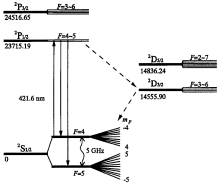
\includegraphics[width=8.6cm, keepaspectratio=true]{sff_1993-87Sr+.eps}
	\caption{Alkali-like energy levels of \Srion{87}{+}. Figure from \cite{sff_1993}.}
\end{figure}

The hyperfine splitting of the $\SLJ{2}{S}{1/2}$ was measured to be \SI{5002368.363(57)}{\kHz}, meaning the magnetic hyperfine constant was determined to be $A = \SI{-1000473.673(11)}{\kHz}$. 

\section{Electronic properties}

Strontium has two principal transitions from the $\nSLJ{5s^2}{1}{S}{0}$ ground state, one at \SI{461}{\nm} and another at \SI{689}{\nm}. 
The \SI{461}{\nm} transition is used for the blue MOT and absorption imaging while the \SI{689}{nm} transition is used for the red MOT and spectroscopy. 

\begin{table}[htbp]
	\centering
	\begin{tabular}{@{}ccccc@{}}
		\toprule
		Isotope						& Lower level									& Upper level					& $\Delta E_\text{iso}$	& Ref	\\
		\midrule
		\Sr{88}						& $\nSLJ{5s^2}{1}{S}{0}$						& $\nSLJ{5s5p}{1}{P}{1}$		&						&		\\
		\Sr{87}						& $\nSLJF{5s^2}{1}{S}{0}{9/2}$					& $\nSLJF{5s5p}{1}{P}{1}{7/2}$	&						&		\\
									&												& $\nSLJF{5s5p}{1}{P}{1}{11/2}$	&						&		\\
									&												& $\nSLJF{5s5p}{1}{P}{1}{9/2}$	&						&		\\
		\Sr{86}						& $\nSLJ{5s^2}{1}{S}{0}$						& $\nSLJ{5s5p}{1}{P}{1}$		&						&		\\
		\Sr{84}						& $\nSLJ{5s^2}{1}{S}{0}$						& $\nSLJ{5s5p}{1}{P}{1}$		&						&		\\
		\bottomrule
	\end{tabular}
	\caption{\label{tab:blue_isotope_shift}xxxxxxxx.}
\end{table}

*************************************************

\begin{table}[H]
\centering
\begin{tabular}{|l|l|l|l|l|}
\hline
Isotope 	& Lower level    				& Upper level 					& Frequency {[}kHz{]} 	& References 						\\ \hline
\Sr{88} 	& $\nSLJ{5s^2}{1}{S}{0}$ 		& $\nSLJ{5s5p}{1}{P}{1}$ 		&                     	& 						           	\\ \hline
\Sr{87} 	& $\nSLJF{5s^2}{1}{S}{0}{9/2}$ 	& $\nSLJF{5s5p}{1}{P}{1}{7/2}$ 	&                     	& 									\\
			& $\nSLJF{5s^2}{1}{S}{0}{9/2}$ 	& $\nSLJF{5s5p}{1}{P}{1}{9/2}$ 	&                     	& 									\\
			& $\nSLJF{5s^2}{1}{S}{0}{9/2}$ 	& $\nSLJF{5s5p}{1}{P}{1}{11/2}$ &                     	&									\\ \hline
\Sr{86} 	& $\nSLJ{5s^2}{1}{S}{0}$ 		& $\nSLJ{5s5p}{1}{P}{1}$ 		&                     	& 									\\ \hline
\Sr{84} 	& $\nSLJ{5s^2}{1}{S}{0}$ 		& $\nSLJ{5s5p}{1}{P}{1}$ 		&                     	&			 						\\ \hline
\end{tabular}
\caption{Isotopic transition frequencies of the 461 nm line.}
\label{blue_iso_freq}
\end{table}

\subsection{Strontium isotope shifts}

Strontium has two principal transitions from the $\nSLJ{5s^2}{1}{S}{0}$ ground state, one at \SI{461}{\nm} and another at \SI{689}{\nm}. 

\subsection{689 nm transition}

\begin{table}[H]
\centering
\begin{tabular}{|c|c|c|l|}
\hline
Isotope						& Lower level									& Upper level										& \multicolumn{1}{c|}{Frequency [\si{kHz}]}							\\ \hline
\multirow{5}{*}{\Sr{88}}	& \multirow{5}{*}{$\nSLJ{5s^2}{1}{S}{0}$}		& \multirow{5}{*}{$\nSLJ{5s5p}{3}{P}{1}$}			& \num{434829121311 +- 10} \cite{Sansonetti_2010, Ferrari_2003}		\\ %\cline{4-4}
							&												&													& \num{434829121300 +- 20} \cite{Courtillot_2005}					\\ %\cline{4-4}
							&												&													& \num{434829121312.334 +- 0.039} \cite{Ido_2005}					\\ %\cline{4-4}
							&												&													& \num{434829121313 +- 20} \cite{Hui_2015}							\\ \cline{4-4}
							&												&													& \num{434829121312.334 +- 0.039}									\\ \hline
\multirow{9}{*}{\Sr{87}}	& \multirow{3}{*}{$\nSLJF{5s^2}{1}{S}{0}{9/2}$}	& \multirow{3}{*}{$\nSLJF{5s5p}{3}{P}{1}{7/2}$}		& \num{434830473270 +- 55} \cite{Sansonetti_2010, Courtillot_2005}	\\ %\cline{4-4}
							&												&													& \num{434830473218 +- 55} \cite{Hui_2015}							\\ \cline{4-4}
							&												&													& \num{434830473244 +- 39}											\\ \cline{2-4}
							& \multirow{3}{*}{$\nSLJF{5s^2}{1}{S}{0}{9/2}$}	& \multirow{3}{*}{$\nSLJF{5s5p}{3}{P}{1}{9/2}$}		& \num{434829343010 +- 50} \cite{Sansonetti_2010, Courtillot_2005}	\\ %\cline{4-4}
							&												&													& \num{434829342986 +- 65} \cite{Hui_2015}							\\ \cline{4-4}
							&												&													& \num{434829343001 +- 40}											\\ \cline{2-4}
							& \multirow{3}{*}{$\nSLJF{5s^2}{1}{S}{0}{9/2}$}	& \multirow{3}{*}{$\nSLJF{5s5p}{3}{P}{1}{11/2}$}	& \num{434827879860 +-55} \cite{Sansonetti_2010, Courtillot_2005}	\\ %\cline{4-4}
							&												&													& \num{434827879826 +- 60} \cite{Hui_2015}							\\ \cline{4-4}
							&												&													& \num{434827879844 +- 41}											\\ \hline
\multirow{3}{*}{\Sr{86}}	& \multirow{3}{*}{$\nSLJ{5s^2}{1}{S}{0}$}		& \multirow{3}{*}{$\nSLJ{5s5p}{3}{P}{1}$}			& \num{434828957494 +- 10} \cite{Sansonetti_2010, Ferrari_2003}		\\ %\cline{4-4}
							&												&													& \num{434828957493 +- 25} \cite{Hui_2015}							\\ \cline{4-4}
							&												&													& \num{434828957493.9 +- 9.3}**										\\ \hline
\Sr{84}						& $\nSLJ{5s^2}{1}{S}{0}$						& $\nSLJ{5s5p}{3}{P}{1}$							& \num{434828769718 +- 111} \cite{Hui_2015}							\\ \hline
\end{tabular}
\caption{Absolute transition frequencies of the 689 nm intercombination line.}
\label{red_iso_freq}
\end{table}


\chapter{Optical Dipole Traps}

Put ODT details here.

\section{Optical Dipole Potential}

**** The derivation below loosely follows that found in \cite{Steck.QuantumAtomOptics, Ludlow2008.PhD} ****

For a two-level atom with ground (excited) state $\ket{g}$ ($\ket{e}$) with energy $E_{g} = \hbar \omega_{g}$ ($E_{e} = \hbar \omega_{e}$), the atomic Hamiltonian $H_{A}$ can be written as
\begin{equation}
	H_{A}	=	\hbar
				\begin{pmatrix}
					\omega_{e}	&	0			\\
					0			&	\omega_{g}
				\end{pmatrix}
\end{equation}
** Somehow introduce $\vb{d}\cdot\vb{E} \rightarrow \Omega \exp(-\iu \omega_{L} t)$ **
Introducing a laser at frequency $\omega$ which couples $\ket{g}$ and $\ket{e}$ and can be represented by
\begin{equation}
	H_{AF}	=	\frac{\hbar}{2}
				\begin{pmatrix}
					0							&	\Omega \cos(\omega t)	\\
					\Omega^{*} \cos(\omega t)	&	0
				\end{pmatrix}
\end{equation}
Using the unitary transformation
\begin{equation}
	U	=	\begin{pmatrix}
				\me^{\iu \omega t}	&	0	\\
				0					&	1
			\end{pmatrix}
\end{equation}
the total (transformed) Hamiltonian for the system can be written as
\begin{equation}
	\widetilde{H}	=		\hbar
							\begin{pmatrix}
								-\Delta												&	\frac{\Omega}{2} \qty(1 + \me^{\iu 2 \omega t})	\\
								\frac{\Omega^{*}}{2} \qty(1 + \me^{-\iu 2 \omega t})	&	\omega_{g}
							\end{pmatrix}
					\approx	\hbar
							\begin{pmatrix}
								-\Delta					&	\frac{\Omega}{2}	\\
								\frac{\Omega^{*}}{2}	&	\omega_{g}
							\end{pmatrix}
\end{equation}
where $\Delta \equiv \omega - \omega_{e}$ and the rotating wave approximation (RWA) was made ** clarify why/how the RWA is done **.

For $\Delta \gg \Omega$, ..... continue deriving...
\chapter{Tips and Tricks}
\label{ap:tips_n_tricks}

Various tips and tricks I picked up over the years. 

\section{Working with (high-power) fibers}

Notes about fibered ODT setup.

Having a fiber inspection scope is super helpful\footnote{We recently acquired a F1MS200U from Fiber Instrument Sales and FS201-PM from Thorlabs.}

\section{Fiber injection lock slave lasers}

We found that using a fiber to couple injection light to a slave laser greatly increased the flexibility and ease-of-use of the slave laser. Fibering the injection light greatly shortens the path lengths compared to free-space injection locking. The fiber also enables easier optimization of the injection lock by using the light back-coupled through the fiber (exiting the ``input'' end) to optimize alignment to the diode. 

\section{Scanning the UV laser}
\label{ap:scanning_uv_laser}

**Talk about how we used to flip-flop sidebands to patch together the $n=98-99$ scan but then the new synthesizer allows us to continue scanning once we hop over the transfer cavity crossing.**

Our current transfer cavity has an FSR of about **\SI{300}{\MHz}** which means the sidebands cross every **\SI{150}{\MHz}**.

\subsection{Switching sidebands to increase scan range}

**Talk about how we used to flip-flop sidebands to patch together the $n=98-99$ scan but then the new synthesizer allows us to continue scanning once we hop over the transfer cavity crossing.**

\subsection{``Continuous'' scanning of the transfer cavity}

**Using the new synthesizer, blah, blah, blah, we no longer have to switch EOM sidebands every FSR/2. 
If we want to scan a few GHz (limited by the synthesizer and RF amplifier ranges) we just need to hop over sideband crossings.**
\chapter{Derivations}

Random derivations I needed for my thesis so I included them here. 

\section{Unitary transformation}

For a unitary transformation $U$ where $\ket*{\psi} = U \ket*{\widetilde{\psi}}$, the Schr\"{o}dinger equation becomes
\begin{equation}
	\iu \hbar \ket*{\dot{\psi}} = H \ket*{\psi}
		\rightarrow \iu \hbar \pdv{t} \left(U \ket*{\widetilde{\psi}}\right) = H \left(U \ket*{\widetilde{\psi}}\right)
\end{equation}
From here, it's pretty easy to obtain the transformed Hamiltonian $\widetilde{H}$
\begin{align}
	\iu \hbar \left(\dot{U} \ket*{\widetilde{\psi}} + U \ket*{\dot{\widetilde{\psi}}}\right) &= H U \ket*{\widetilde{\psi}}	\nonumber \\
	\iu \hbar U \ket*{\dot{\widetilde{\psi}}} &= H U \ket*{\widetilde{\psi}} - \iu \hbar \dot{U} \ket*{\widetilde{\psi}}	\nonumber \\
	\iu \hbar \ket*{\dot{\widetilde{\psi}}} &= \left(U^\dag H U - \iu \hbar U^\dag \dot{U}\right) \ket*{\widetilde{\psi}}	\nonumber \\
	\iu \hbar \ket*{\dot{\widetilde{\psi}}} &= \widetilde{H} \ket*{\widetilde{\psi}}
\end{align}
where $\widetilde{H} = U^\dag H U - \iu \hbar U^\dag \dot{U}$ for the transformed state $\ket*{\widetilde{\psi}} = U^\dag \ket*{\psi}$.

%\include{append-a}
%\appendix
%\addcontentsline{toc} {chapter}{\numberline {}Appendix A}
%\include{append-a}
%\include{append-b}
%\addcontentsline{toc} {chapter}{\numberline {}Bibliography}{}
%\include{biblio}

%%%%%%%%%%%%%%%%%%%%%%%%%%%%%%%%%%%%%%%%%%%%%%%%%%%%%%%%%%%%%%%%%%%
%%%%	Bibliography
%%%%%%%%%%%%%%%%%%%%%%%%%%%%%%%%%%%%%%%%%%%%%%%%%%%%%%%%%%%%%%%%%%%

%\bibliographystyle{ieeetr}
%\bibliography{bibliography}
\addcontentsline{toc}{chapter}{Bibliography}
\printbibliography

\end{document}
